\section{Java}
Java je jedním z nejpoužívanějších a nejpopulárnějších počítačových programovacích jazyků na světě. Syntaxe tohoto jazyka se řadí k těm jednodužším, avšak jeho použití je velmi rozsáhlé. V Java se programují čipové karty, mobilní a desktopové aplikace, i velké podnikové a informační systémy. Java je jazyk multiplatformní a díky tomu je jej možné použít ná různých operačních systémech. Java je vyvíjena jako OpenSource. Java se objevuje ve třech základních edicích:


\subsection{Java platformy}
Jazyk Java je společně s virtuálním strojem a knihovnami vydáván ve čtyřech platformách, kde každá má své speciální určení.

\subsubsection{Java SE}
Základní platforma pro vývoj desktopových a jednodužších serverových aplikací. V součané době je poslední vydaná verze Java SE 8u25.

\subsubsection{Java EE}
Nádstavba nad Java SE obsahující speciální knihovny pro vývoj a provoz podnikových aplikací a informačních systémů. V součané době je poslední vydaná verze Java EE 7.

\subsubsection{Java ME (Micro Edition)}
Podmnožina Java SE pro vývoj aplikací pro malá zařízení jako jsou mikrokontroléry sensory, mobilní telefony, set-top boxy, tiskárny a další. V součané době je poslední vydaná verze Java ME 8.1.

\subsubsection{Java Card}
Verze určená pro vývoj aplikací určených pro čipové karty a pro zařízení s limitovanou pamětí a schopností zpracovávání. Příkladem mohou být SIM karty pro mobilní zařízení nebo čipové karty pro ATM bankomaty. V součané době je poslední vydaná verze Java Card 3.0.4.

\subsection{Vývojářské sady}
Možnosti jak Javu stáhnout jsou dvě. Jedná se o balík se kterým lze pouze spouštět aplikace Java (JRE) nebo balík který slouží pro vývoj (JDK).

\subsubsection{Java JRE (Java Runtime Environment)}
Běhové prostředí Javy, které poskytuje vše potřebné pro suštění java aplikací. Součástí je virtuální stroj javy a potřebné knihovny.

\subsubsection{Java JDK (Java Development Kit)}
Někdy se také označuje SDK (Software Development Kit). Jedná se o sadu JRE doplněnou o vyvojářské nástroje (překladač, generátor dokumentace, ladící nástroje a další).

\begin{figure}[h!]
    \centering
    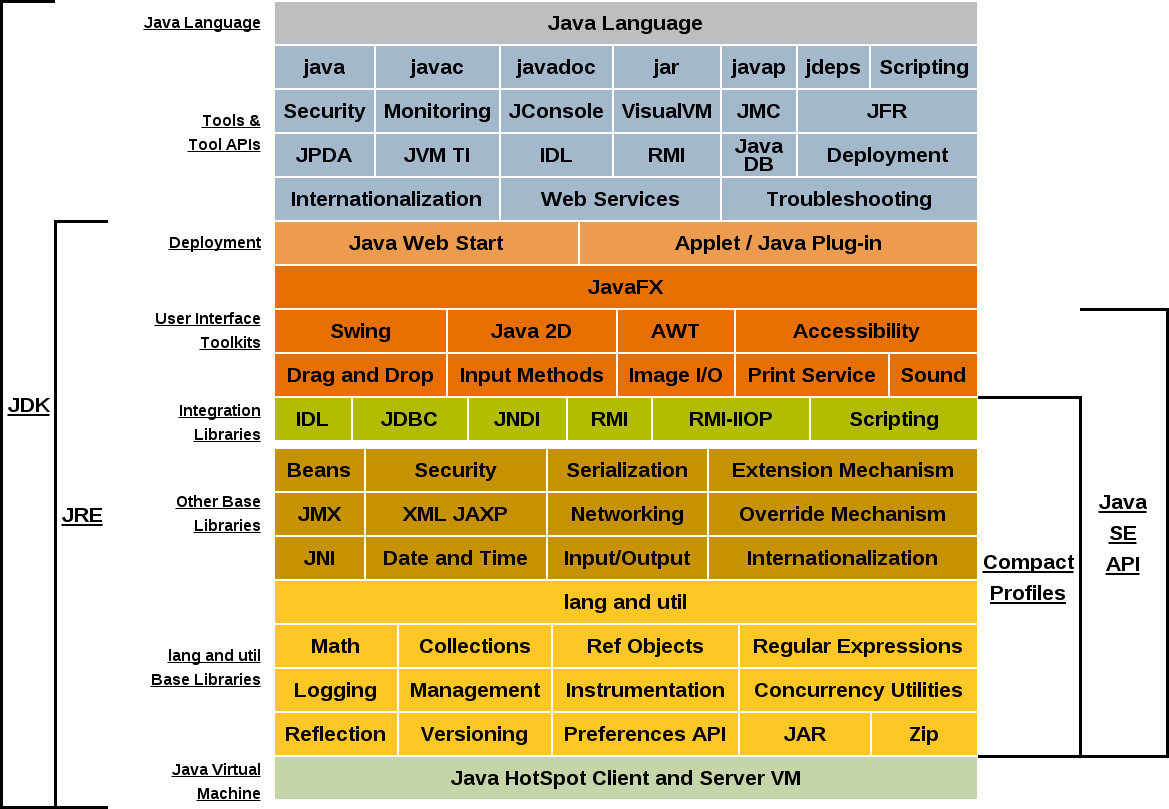
\includegraphics[scale=0.3]{fig/java_jdk.jpg}
    \caption{Java SE JDK 1.8}
\end{figure}



\section{Android}



\section{Gradle}


\section{JBoss Drools}

  \subsection{Drools Expert}

  \subsection{OptaPlanner}


\section{Vehicle routing problem}

%\subsection{History}
%V následující tabulce je stručně popsána historie programovacího jazyku Java: \\
%\\
%\begin {table}[h!]
%\begin{tabular}{|l|l|l|}[h]
%\hline
%    {\bf Název} & {\bf Datum} & {\bf Poznámka}  \\
%    \hline \hline
%    Oak         & 1991                  & a     \\
%    JDK         & 1995                  & a     \\
%    JDK 1.0     & January 23rd, 1996    & a     \\
%    JDK 1.1     & February 19th, 1997   & a     \\
%    JPE         & May, 1998             & a \\
%    J2SE 1.2    & December 8th, 1998    & a     \\
%    J2EE 1.2    & December 12, 1999     & a     \\
%    J2SE 1.3    & May 8th, 2000         & a     \\
%    J2EE 1.3    & September 24, 2001    & a \\
%    J2SE 1.4    & February 6th, 2002    & a     \\
%    J2EE 1.4    & November 11, 2003     & a \\
%    J2SE 5.0    & September 30th, 2004  & a     \\
%    Java EE 5   & May 11, 2006          & a \\
%    Java SE 6   & December 11th, 2006   & a     \\
%    Java EE 6   & December 10, 2009     & a \\
%    Java SE 7   & July 28th, 2011       & a     \\
%    Java EE 7   & June 12, 2013         & a \\
%    Java SE 8   & March 18th, 2014      & a     \\
%  \hline
%\end{tabular}
%\caption{Historie Javy}
%\end{table}




